
\title{Status and Technological Assessment of Si/SiGe Spin Qubits}
\date{\today}



\maketitle

% Reset counter for Q/A structure


\section{Companies Pursuing Quantum Computers Based on Si/SiGe Qubit Technology}

Several academic, government, and commercial entities are actively pursuing quantum computers based on Si/SiGe spin qubits \cite{ref1, ref2, ref5, ref6, ref10}.

\begin{itemize}
    \item \textbf{Intel Corporation} is a prominent commercial entity, focusing on scalable qubit architectures \cite{ref5}, the development of cryogenic control chips like \textbf{Horse Ridge} (operating at 3K) \cite{ref6}, and demonstrating the fabrication of 12-spin-qubit arrays on a standard 300 mm manufacturing line \cite{ref10}.
    \item \textbf{IBM} is involved via \textbf{IBM Research-Zürich}, which has contributed to work on hole spin qubits in FinFETs \cite{ref6}.
    \item \textbf{TU Delft} researchers have conducted collaborative work, sometimes with support from Intel \cite{ref2}.
    \item \textbf{HRL Laboratories, LLC} has provided the necessary Si/SiGe heterostructures for some key experiments.
    \item \textbf{Sandia National Laboratories} has served as a research partner in various projects \cite{ref1}.
\end{itemize}

\section{Type of Quantum Computers Exploited with Si/SiGe Qubits}

The technology primarily supports \textbf{gate-based digital quantum computers} and \textbf{analog quantum simulators} \cite{ref2, ref9}. The gate-based approach follows the quantum circuit model, utilizing universal sets of gates (e.g., single-qubit rotations and two-qubit CNOT gates) to execute arbitrary quantum algorithms \cite{ref2}.

\subsection{Gate/Pulse-Based Control}
The control mechanism employed is \textbf{pulse-based} \cite{ref2, ref9}.
\begin{itemize}
    \item \textbf{Single-qubit gates} are achieved by applying tailored microwave pulses to drive Electron Spin Resonance (ESR) or Electric Dipole Spin Resonance (EDSR) \cite{ref2, ref9}.
    \item \textbf{Two-qubit gates} (e.g., CNOT and controlled-phase (CPHASE or CZ)) are implemented by using fast voltage pulses to precisely control the exchange interaction between adjacent spins \cite{ref1, ref2, ref9}.
\end{itemize}

\subsection{Digital/Analog Computation}
The technology has demonstrated versatility in both digital and analog computation \cite{ref9}.
\begin{itemize}
    \item \textbf{Digital Computation:} Demonstrations include foundational quantum algorithms (Deutsch-Josza, Grover search \cite{ref2}) and application methods like the Variational Quantum Eigensolver (VQE) \cite{ref9}.
    \item \textbf{Analog Computation:} Analog quantum simulations focusing on condensed matter systems have been successfully performed using three to four spin qubits \cite{ref9}.
\end{itemize}
\emph{Note:} The provided materials do not indicate the use of Si/SiGe spin qubits for quantum annealing \cite{ref8, ref9}.

\section{Availability Through Cloud Computing Platforms}

Si/SiGe spin qubit technology is \textbf{not currently available} to the general public or commercial users via established cloud computing platforms (e.g., AWS Braket, Microsoft Azure Quantum, Google Cloud). These platforms currently prioritize superconducting, trapped-ion, and photonic technologies.

The primary reasons for this current lack of commercial cloud access are:
\begin{itemize}
    \item \textbf{Focus on Foundational Challenges:} Research efforts are concentrated on overcoming fundamental hardware obstacles related to scaling, achieving qubit uniformity, and improving fidelity, aligning with the long-term goal of leveraging CMOS manufacturing for millions of qubits.
    \item \textbf{The ``Variability'' Problem:} A significant challenge is the nanoscale fabrication variation that requires complex and often manual ``tuning'' of operating voltages for each gate-defined quantum dot. Automated tuning, which is a prerequisite for robust cloud service, remains an active area of research.
    \item \textbf{Alternative Access Models:} Instead of commercial cloud offerings, availability is limited to direct research collaborations. For instance, Intel provides its research chips, such as the 12-qubit Tunnel Falls processor, to select academic and governmental partners to foster community R\&D efforts.
\end{itemize}

\section{Status of Qubit Hardware Development}

Hardware development for Si/SiGe spin qubits has achieved significant milestones in scalability, fidelity, and industrial compatibility \cite{ref1, ref4, ref9, ref10, ref11}.

\subsection{Key Milestones}
\begin{itemize}
    \item \textbf{Qubit Count:} Processors with up to six working qubits have been demonstrated \cite{ref11}. Intel has also fabricated chips featuring 12-quantum-dot linear arrays, marking the largest reported qubit count in a single spin-qubit device \cite{ref10}.
    \item \textbf{Fidelities:} High fidelities have been achieved across all critical operations:
    \begin{itemize}
        \item \textbf{Single-Qubit Gates:} Fidelities commonly exceed 99\% \cite{ref1}, with reports reaching up to $99.96\%$ \cite{ref9}. A six-qubit processor showed average single-qubit gate fidelities between $99.77\%$ and $99.96\%$ \cite{ref11}.
        \item \textbf{Two-Qubit Gates:} A CPHASE gate fidelity surpassing $99.8\%$ has been demonstrated \cite{ref1}, alongside other work showing a fidelity of $99.5\%$ \cite{ref9}. Bell state fidelities range from $88-96\%$ in recent demonstrations \cite{ref11}.
        \item \textbf{SPAM (State Preparation and Measurement) Errors:} Total SPAM errors are reported below $3\%$ \cite{ref1}, with qubit visibilities ranging from $93.5-98\%$ \cite{ref11}.
    \end{itemize}
    \item \textbf{Scalability and Fabrication:} The technology is fully compatible with industrial Complementary-Metal-Oxide-Semiconductor (CMOS) fabrication processes \cite{ref2, ref5, ref7, ref10}. Intel specifically demonstrated fabrication on a $300$ mm wafer line using advanced lithography (immersion and EUV), yielding reproducible arrays where $96\%$ of devices successfully tuned to the single-electron regime \cite{ref10}.
    \item \textbf{Operating Temperature:} While most experiments require temperatures below 100 mK \cite{ref5}, progress on ``hot qubits'' includes the demonstration of hole spin qubit operation above 1K and even above 4K \cite{ref6}.
\end{itemize}

\section{Implementation of Computations and Simulations}

Computations are implemented through a sequential process of initialization, gate application, and readout, all controlled via electrical pulses \cite{ref2, ref9, ref11}.

\begin{enumerate}
    \item \textbf{Initialization:} Qubits are prepared in a well-defined initial state. Methods include energy-selective tunneling (loading an electron into its ground spin state) or Pauli Spin Blockade (PSB), which utilizes spin selection rules in a double quantum dot \cite{ref2, ref9}.
    \item \textbf{Gate Application:} The algorithm is executed by applying the determined sequence of gates.
    \begin{itemize}
        \item \textbf{Single-qubit gates} are applied by sending microwave pulses tuned to the qubit's resonance frequency (ESR or EDSR) \cite{ref1, ref2}.
        \item \textbf{Two-qubit entangling gates} (CNOT, CZ) are realized by pulsing the voltage on electrostatic gates, temporarily turning on the exchange interaction between adjacent spins \cite{ref1, ref2, ref9}.
    \end{itemize}
    \item \textbf{Readout:} The final spin state is measured. This is typically done by mapping the spin state onto a charge state using PSB or spin-selective tunneling \cite{ref2, ref9}. The resulting charge configuration is detected by a highly sensitive nearby charge sensor \cite{ref2, ref9}. For internal qubits, Quantum Non-Demolition (QND) measurements are sometimes used to map the state onto a dedicated readout qubit \cite{ref11}.
\end{enumerate}

\section{Use and Applications of the Quantum Computer}

The primary current use of Si/SiGe quantum computers is serving as programmable processors to benchmark quantum algorithms and simulate complex quantum systems \cite{ref2, ref9}.

\subsection{Use-Case Example: Foundational Algorithm Demonstration}
A key use-case is the implementation of established quantum algorithms on small-scale silicon processors \cite{ref2}. Watson et al. successfully used a programmable processor based on a natural Si/SiGe double quantum dot to execute both the \textbf{Deutsch-Josza} and the \textbf{Grover search algorithms} \cite{ref2}. While these are verification algorithms, their success demonstrates the necessary universal control of the hardware required for future complex computations.

\subsection{Other Demonstrated Applications}
\begin{itemize}
    \item \textbf{Analog Simulation:} Analog quantum simulations of condensed matter physics using three to four qubits \cite{ref9}.
    \item \textbf{Quantum Algorithms:} Execution of the Variational Quantum Eigensolver (VQE) method \cite{ref9}.
    \item \textbf{Entanglement Verification:} Preparation of Greenberger-Horne-Zeilinger (GHZ) states across three qubits to verify multi-qubit entanglement and control \cite{ref11}.
\end{itemize}
These applications serve to verify hardware capabilities and benchmark performance toward solving practical, real-world problems \cite{ref2, ref9}.
\section{Fulfillment of the DiVincenzo Criteria}
The Si/SiGe spin qubit technology is evaluated against the five requirements for a functional quantum computer, as laid out by DiVincenzo \cite{ref12}. The following table highlights and describes each individually.

\begin{table}[H]
    \centering
    \caption{Assessment of Si/SiGe Spin Qubits against DiVincenzo Criteria}
    \begin{tabular}{|p{0.35\textwidth}|c|p{0.50\textwidth}|}
        \hline
        \textbf{Criterion} & \textbf{Assessment} & \textbf{Explanation} \\
        \hline
        \multicolumn{3}{|l|}{\textbf{1. A scalable physical system with well-characterized qubits.}} \\
        \hline
        \hspace{5mm} \emph{Scalability (Qubit Number)} & Partially Fulfilled & Functional processors up to six qubits \cite{ref11} and fabricated 12-dot linear arrays \cite{ref10} show scaling progress, but massive qubit counts are yet to be achieved \cite{ref2, ref9}. \\
        \hline
        \hspace{5mm} \emph{Scalability (Technological Infrastructure)} & Yes & A primary strength. The technology is inherently compatible with industrial CMOS manufacturing processes, including 300 mm wafers and EUV lithography, providing a clear path to mass production \cite{ref2, ref5, ref7, ref10}. \\
        \hline
        \hspace{5mm} \emph{Well-Characterized Qubits} & Yes & Qubits are encoded in the spin states of single electrons in quantum dots. The Hamiltonians, exchange interactions, and couplings to external fields are well understood and modeled \cite{ref9, ref12}. \\
        \hline
        \textbf{2. The ability to initialize the state of the qubits to a simple fiducial state.} & Yes & High-fidelity initialization is achieved via energy-selective tunneling from a reservoir \cite{ref9}, Pauli Spin Blockade (PSB) \cite{ref2, ref9}, or real-time feedback based on measurement \cite{ref11}. \\
        \hline
        \textbf{3. Long relevant decoherence times, much longer than the gate operation time.} & Yes & Single-qubit gates ($\sim$ tens to hundreds of nanoseconds) and two-qubit gates ($\sim$ tens of nanoseconds) \cite{ref9, ref11} are much faster than Hahn echo coherence times (T$_2$), which can exceed 100~$\mu$s in isotopically enriched silicon \cite{ref4, ref9}. \\
        \hline
        \textbf{4. A "universal" set of quantum gates.} & Yes & Universality is demonstrated using single-qubit rotations (ESR/EDSR microwave pulses \cite{ref2, ref9}) and two-qubit entangling gates (CNOT/CZ via pulsed exchange interaction \cite{ref1, ref2, ref9}). \\
        \hline
        \textbf{5. A qubit-specific measurement capability.} & Yes & High-fidelity, qubit-specific readout is achieved primarily through spin-to-charge conversion, detected by proximal charge sensors (SET or QPC) \cite{ref2, ref9}. Quantum Non-Demolition (QND) measurements are used for internal array qubits \cite{ref11}. \\
        \hline
    \end{tabular}
\end{table}

\section{Benefits and Challenges}

\subsection{Benefits}
The Si/SiGe spin qubit platform offers several compelling advantages:
\begin{itemize}
    \item \textbf{Scalability and Density:} Quantum dots are small ($\sim$100~nm), allowing for high-density integration \cite{ref2, ref9}.
    \item \textbf{CMOS Compatibility:} The primary benefit is alignment with established, high-volume CMOS manufacturing, facilitating reproducible device creation on 300~mm industrial wafer lines \cite{ref2, ref5, ref9, ref10}.
    \item \textbf{Coherence:} In isotopically purified silicon, the electron spins are isolated from nuclear spin noise, leading to inherently long quantum coherence times \cite{ref9, ref12}.
    \item \textbf{Control:} Control relies on fast, precise electrical voltage and microwave pulses, leveraging mature electronics technology \cite{ref2, ref7}. High-fidelity single- and two-qubit operations are demonstrated \cite{ref1, ref4, ref9}.
\end{itemize}

\subsection{Challenges}
The key obstacles currently faced by the technology include:
\begin{itemize}
    \item \textbf{Charge Noise:} While spins are robust, their electrical control mechanisms (especially the exchange interaction) are highly susceptible to semiconductor electric field noise, which remains a dominant source of gate error and decoherence \cite{ref4, ref9}.
    \item \textbf{Device Variability and Tuning:} Nanoscale fabrication variations result in slightly different properties for each quantum dot, necessitating a complex, high-precision manual calibration ("tuning") process for every individual qubit, hindering large-scale automation \cite{ref5}.
    \item \textbf{Crosstalk and Connectivity:} Managing the wiring fan-out and preventing microwave crosstalk between dense, adjacent qubits is a significant engineering hurdle that grows exponentially with qubit count \cite{ref2, ref5, ref9, ref11}.
    \item \textbf{Valley Degeneracy:} The multiple valley states in the silicon conduction band are close to the qubit energy levels, complicating stable qubit control and readout \cite{ref2}.
\end{itemize}

\section{Prospect for Useful Quantum Advantage}


\begin{enumerate}
    \item \textbf{Near-Term (NISQ Era):} With processors in the tens of qubits, the technology can immediately be applied to \textbf{bespoke quantum simulations}. This includes modeling condensed matter systems or quantum chemistry problems that are already intractable for the most powerful classical supercomputers today \cite{ref8, ref9}.
    \item \textbf{Long-Term (Fault-Tolerant Era):} The core promise is the ability to scale up to large, error-corrected machines capable of executing algorithms that offer exponential speedups, such as factoring (Shor's algorithm) or advanced optimization problems \cite{ref12}.
\end{enumerate}
The successful demonstration of foundational algorithms like Grover's search and VQE on current silicon hardware confirms the necessary quantum control is in place to work toward these goals \cite{ref2, ref9}.

\section{Prospects for Error Correction}

The prospects for implementing quantum error correction (QEC) are \textbf{very strong} \cite{ref12}. QEC is the foundation of fault tolerance, and it requires the physical gate error rate to be below a certain accuracy threshold (often cited around 1\% or ideally $10^{-4}$ to $10^{-5}$) \cite{ref5, ref12}.

\begin{itemize}
    \item \textbf{High Fidelity Achieved:} Si/SiGe spin qubits have already surpassed these critical thresholds. Single-qubit fidelities exceed $99.9\%$ \cite{ref4}, and two-qubit fidelities have reached $99.8\%$ \cite{ref1}.
    \item \textbf{Compatibility with Codes:} This level of performance is sufficient to support common QEC protocols, such as the surface code \cite{ref1, ref9}.
    \item \textbf{Scaling Challenge:} While the gate quality is high enough for error correction, the remaining challenge is the immense scaling requirement: hundreds or thousands of physical qubits must be reliably controlled to encode a single, robust logical qubit \cite{ref5, ref12}.
\end{itemize}

\section{Path to Universal Fault-Tolerant Quantum Computing}

The Si/SiGe spin qubit technology offers a direct, albeit challenging, path toward creating a universal fault-tolerant quantum computer:

\begin{enumerate}
    \item \textbf{Universal Gate Set:} The demonstrated high-fidelity single- and two-qubit gates already provide the universal control required for general-purpose quantum computation \cite{ref2, ref9, ref12}.
    \item \textbf{Achieving Fault Tolerance:} This is implemented by actively utilizing the high-fidelity gates to execute quantum error correction codes (like the surface code) that protect the stored quantum information from errors \cite{ref1, ref9}.
    \item \textbf{Leveraging Industrial Scale:} The core strategy for scaling is the use of 300 mm CMOS fabrication lines \cite{ref10}. This manufacturing capability provides the highest potential for producing the millions of physical qubits required for large-scale, fault-tolerant computation in highly uniform 2D arrays \cite{ref2, ref9}.
    \item \textbf{Engineering Integration:} Success hinges on solving engineering problems such as co-integrating the classical control and readout electronics (e.g., cryo-CMOS) onto the same package or chip as the quantum array, managing thermal load, and automating the required calibration process for millions of individual qubits \cite{ref2, ref5}.
\end{enumerate}


\section{Performance Metrics and Error Sources}

\subsection{Number of Qubits}
Current development efforts have demonstrated notable progress in scaling the number of qubits:
\begin{itemize}
    \item The largest reported count in a single spin-qubit device is a \textbf{12-quantum-dot (12QD) linear array} fabricated by Intel \cite{ref10}.
    \item A fully universal \textbf{six-qubit quantum processor} has been successfully fabricated and operated \cite{ref11}.
    \item A functional \textbf{four-qubit processor} has been demonstrated using germanium quantum dots \cite{ref9}.
\end{itemize}

\subsection{Gate Fidelities and Times}

The core performance metrics for single- and two-qubit operations are summarized below:

\begin{table}[!htb]
    \centering
    \caption{Summary of Key Operational Metrics for Si/SiGe Spin Qubits}
    \label{tab:metrics}
    \begin{tabular}{|l|c|c|}
        \hline
        \textbf{Metric} & \textbf{Achieved Fidelity (\%)} & \textbf{Typical Time} \\
        \hline
        Single-Qubit Gate (1Q) & $99.926 \pm 0.002$ \cite{ref4} & 60--120 ns ($\pi/2$ to $\pi$ rotations) \cite{ref4} \\
        \hline
        Two-Qubit Gate (2Q) (CPHASE) & $> 99.8$ \cite{ref1, ref9} & 40 ns \cite{ref1} \\
        \hline
        State Preparation (Initialization) & $99.4$ (max reported) \cite{ref1} & 660 ns (using feedback) \cite{ref11} \\
        \hline
        Readout (Measurement) & $> 99.97$ (max reported) \cite{ref11} & $\sim 10$ $\mu$s \cite{ref11} \\
        \hline
    \end{tabular}
\end{table}

\subsubsection{Single-Qubit Gate Performance}
Fidelity for single-qubit gates (1Q) averages $\mathbf{99.926 \pm 0.002\%}$ in isotopically enriched silicon \cite{ref4}. Gate times are fast, with $\pi/2$ rotations achieved in approximately $\mathbf{60~ns}$ and $\pi$ rotations in $\mathbf{120~ns}$ \cite{ref4}.

\subsubsection{Two-Qubit Gate Performance}
A controlled-phase (CPHASE or CZ) two-qubit gate fidelity exceeding $\mathbf{99.8\%}$ has been demonstrated \cite{ref1, ref9}. This high fidelity was achieved with a fast gate time of $\mathbf{40~ns}$ \cite{ref1}.

\subsection{Decoherence Time}
Coherence times vary based on the measurement protocol and the specific spin used (electron or nuclear).
\begin{itemize}
    \item \textbf{T\textsubscript{1} (Relaxation Time):} For donor qubits, the relaxation time T\textsubscript{1} is above \textbf{one second} at 4 K \cite{ref5}.
    \item \textbf{T\textsubscript{2}\textsuperscript{*} (Dephasing Time):} Measured using Ramsey interference, T\textsubscript{2}\textsuperscript{*} reached $\mathbf{20~\mu s}$ in an isotopically enriched Si/SiGe quantum dot \cite{ref4}.
    \item \textbf{T\textsubscript{2} (Coherence Time):} Using a Hahn echo sequence, the coherence time T\textsubscript{2} was measured at $\mathbf{99 \pm 4~\mu s}$ \cite{ref4}. With CPMG dynamical decoupling, this time was extended significantly to $\mathbf{3.1~ms}$ for electron spins \cite{ref4}, and over $\mathbf{30~seconds}$ for donor nuclear spins \cite{ref2}.
\end{itemize}

\subsection{Preparation and Readout Fidelity}
Both initialization and measurement processes have achieved high fidelities:
\begin{itemize}
    \item \textbf{Preparation Fidelity and Time:} Initialization fidelities up to $\mathbf{99.4\%}$ have been reported \cite{ref1}. For initialization based on measurement with real-time feedback, the latency is $\mathbf{660~ns}$ \cite{ref11}.
    \item \textbf{Readout Fidelity and Time:} Measurement fidelity has reached $\mathbf{99.8\%}$ and even exceeded $\mathbf{99.97\%}$ using Pauli Spin Blockade \cite{ref1, ref11}. Readout times are typically on the order of $\mathbf{10~\mu s}$ \cite{ref11}.
\end{itemize}

\subsection{Main Sources of Error}
The dominant limitations on fidelity and coherence in Si/SiGe spin qubits are:
\begin{itemize}
    \item \textbf{Charge Noise:} Fluctuations in the local electric field are the primary limiting source of decoherence, particularly affecting the exchange interaction used for two-qubit gates and the EDSR control fields \cite{ref4, ref9}.
    \item \textbf{Hyperfine Interaction:} Interaction with surrounding nuclear spins (specifically the minority \textsuperscript{29}Si isotope) causes electron spin dephasing. This error is largely mitigated by using isotopically purified silicon (enriched \textsuperscript{28}Si) \cite{ref2, ref4, ref9}.
    \item \textbf{Valley Splitting:} The presence of low-lying valley states in the silicon conduction band introduces complexity in qubit control and can interfere with the spin blockade readout mechanism \cite{ref2}.
    \item \textbf{Crosstalk:} In large arrays, unintended microwave control signals or magnetic field effects between adjacent qubits lead to gate errors, requiring careful physical design and tuning \cite{ref3}.
\end{itemize}

\subsection{Highest Quantum Volume Achieved}
In simulation, using literature-derived parameter ranges and the IBM QV protocol, the LHS configuration \texttt{lhs\_sample\_0002} achieved a maximum passing width of $m^*=11$, corresponding to a simulated Quantum Volume of $\mathrm{QV}=2048$. Other sampled configurations passed up to $m=5$ (QV$=32$) or $m=7$ (QV$=128$). Full methodology and results are detailed in Appendix~\ref{app:qv-campaign}.



% Include simulation appendix with QV campaign details
\clearpage
\appendix
\section{Simulation-based Quantum Volume Estimation for Si/SiGe (Campaign Appendix)}\label{app:qv-campaign}

This appendix documents how simulated Quantum Volume (QV) was estimated from literature-derived device parameters and summarizes the results of a small Latin Hypercube Sampling (LHS) campaign. The goal is to show, in a controlled simulation setting, how realistic ranges of single- and two-qubit fidelities, coherence times, crosstalk, and SPAM parameters translate into IBM-style QV outcomes.

\subsection{Methodology and decision rule}
We follow the IBM Quantum Volume protocol for width $m$ (and equal depth $m$):
\begin{enumerate}
    \item For each width $m$, generate $N=100$ random square circuits following the QV prescription and transpile/schedule subject to nearest-neighbor constraints.
    \item For each circuit, compute the heavy-output probability (HOP) by first obtaining the ideal (noiseless) output probabilities and identifying ``heavy'' bitstrings with probability above the median; then run a noisy simulation with $5{,}000$ shots and estimate the observed heavy-output frequency.
    \item Aggregate across the $N$ circuits to obtain a sample mean HOP and a 95\% bootstrap confidence interval $[\mathrm{CI}_\mathrm{low},\,\mathrm{CI}_\mathrm{high}]$.
    \item Pass criterion (per IBM): declare width $m$ as passed if both the sample mean and the lower 95\% CI bound exceed $2/3$.
\end{enumerate}
The achieved Quantum Volume is then defined as $\mathrm{QV} = 2^{m^*}$ for the largest width $m^*$ that passes. Because finite-sample statistics can introduce mild non-monotonicity (e.g., an occasional pass at $m{+}1$ when $m$ narrowly fails), we report the maximum passing width observed and indicate any such occurrences explicitly.

\subsection{Noise model construction from literature parameters}
Device parameters were sampled via LHS from ranges compiled from recent Si/SiGe spin-qubit literature (see main text and \texttt{campaign\_manifest.json}). The simulator constructs a composite noise model with coherent and stochastic components using the following mappings:
\begin{itemize}
    \item Average fidelity to depolarizing probability:
    \[
      p_{1\mathrm{Q}} = 2\,(1 - F_1),\qquad p_{2\mathrm{Q}} = \tfrac{4}{3}\,(1 - F_2).
    \]
    \item Amplitude and phase damping during a gate of duration $\tau$:
    \[
      p_\mathrm{amp} = 1 - e^{-\tau/T_1},\qquad p_\phi = 1 - e^{-\tau/T_\phi},\quad \text{with } \tfrac{1}{T_\phi} = \tfrac{1}{T_2} - \tfrac{1}{2T_1}.
    \]
    \item Quasi-static detuning to model slow drift via $T_2^*$:
    \[
      \Delta \sim \mathcal{N}\!\bigl(0,\,\sigma^2\bigr),\quad \sigma = \tfrac{\sqrt{2}}{T_2^*},
    \]
    sampled once per circuit.
\end{itemize}
SPAM, control crosstalk, and residual ZZ coupling are included per-sample using the values in each YAML configuration; two-qubit gate time is fixed at 40\,ns; single-qubit gate times are sampled in the 60--70\,ns range.

\subsection{Campaign setup}
The campaign evaluated $5$ configurations (\texttt{lhs\_sample\_0000} through \texttt{0004}) drawn by LHS over the ranges listed in the manifest (e.g., $F_2\in[0.92,\,0.9981]$, $T_2\in[245\,\mathrm{ns},\,3.1\,\mathrm{ms}]$, $T_2^*\in[0.36,\,20]$\,$\mu$s, control crosstalk $\in[0.44\%,\,1.85\%]$). Each configuration simulated widths $m=2,\dots,12$ with $N=100$ circuits per width and $5{,}000$ shots per circuit.

\subsection{Results summary}
Table~\ref{tab:qv-summary} summarizes the simulated QV outcomes. The maximum passing width $m^*$ and corresponding QV are reported, together with the first failing width when applicable.

\begin{table}[!htb]
  \centering
  \caption{Simulated QV outcomes by LHS configuration (pass threshold $2/3$ with 95\% CI).}
  \label{tab:qv-summary}
  \begin{tabular}{lcccc}
    \hline
    Configuration & Max pass $m^*$ & QV $=2^{m^*}$ & First fail width & Notes \\
    \hline
    lhs\_sample\_0000 & 5 & 32 & 6 & Monotonic (2--5 pass, 6+ fail) \\
    lhs\_sample\_0001 & 7 & 128 & 6 & 6 fails on CI, 7 passes (finite-sample non-monotonic) \\
    lhs\_sample\_0002 & 11 & 2048 & 12 & Strong, passes 2--11, 12 fails (mean and CI) \\
    lhs\_sample\_0003 & 5 & 32 & 6 & Monotonic (2--5 pass, 6+ fail) \\
    lhs\_sample\_0004 & 5 & 32 & 6 & Monotonic (2--5 pass, 6+ fail) \\
    \hline
  \end{tabular}
\end{table}

Figure~\ref{fig:qv-overview} illustrates the campaign-wide comparison, and Figure~\ref{fig:qv-waterfall} shows the pass/fail transitions by width.

\begin{figure}[!htb]
  \centering
  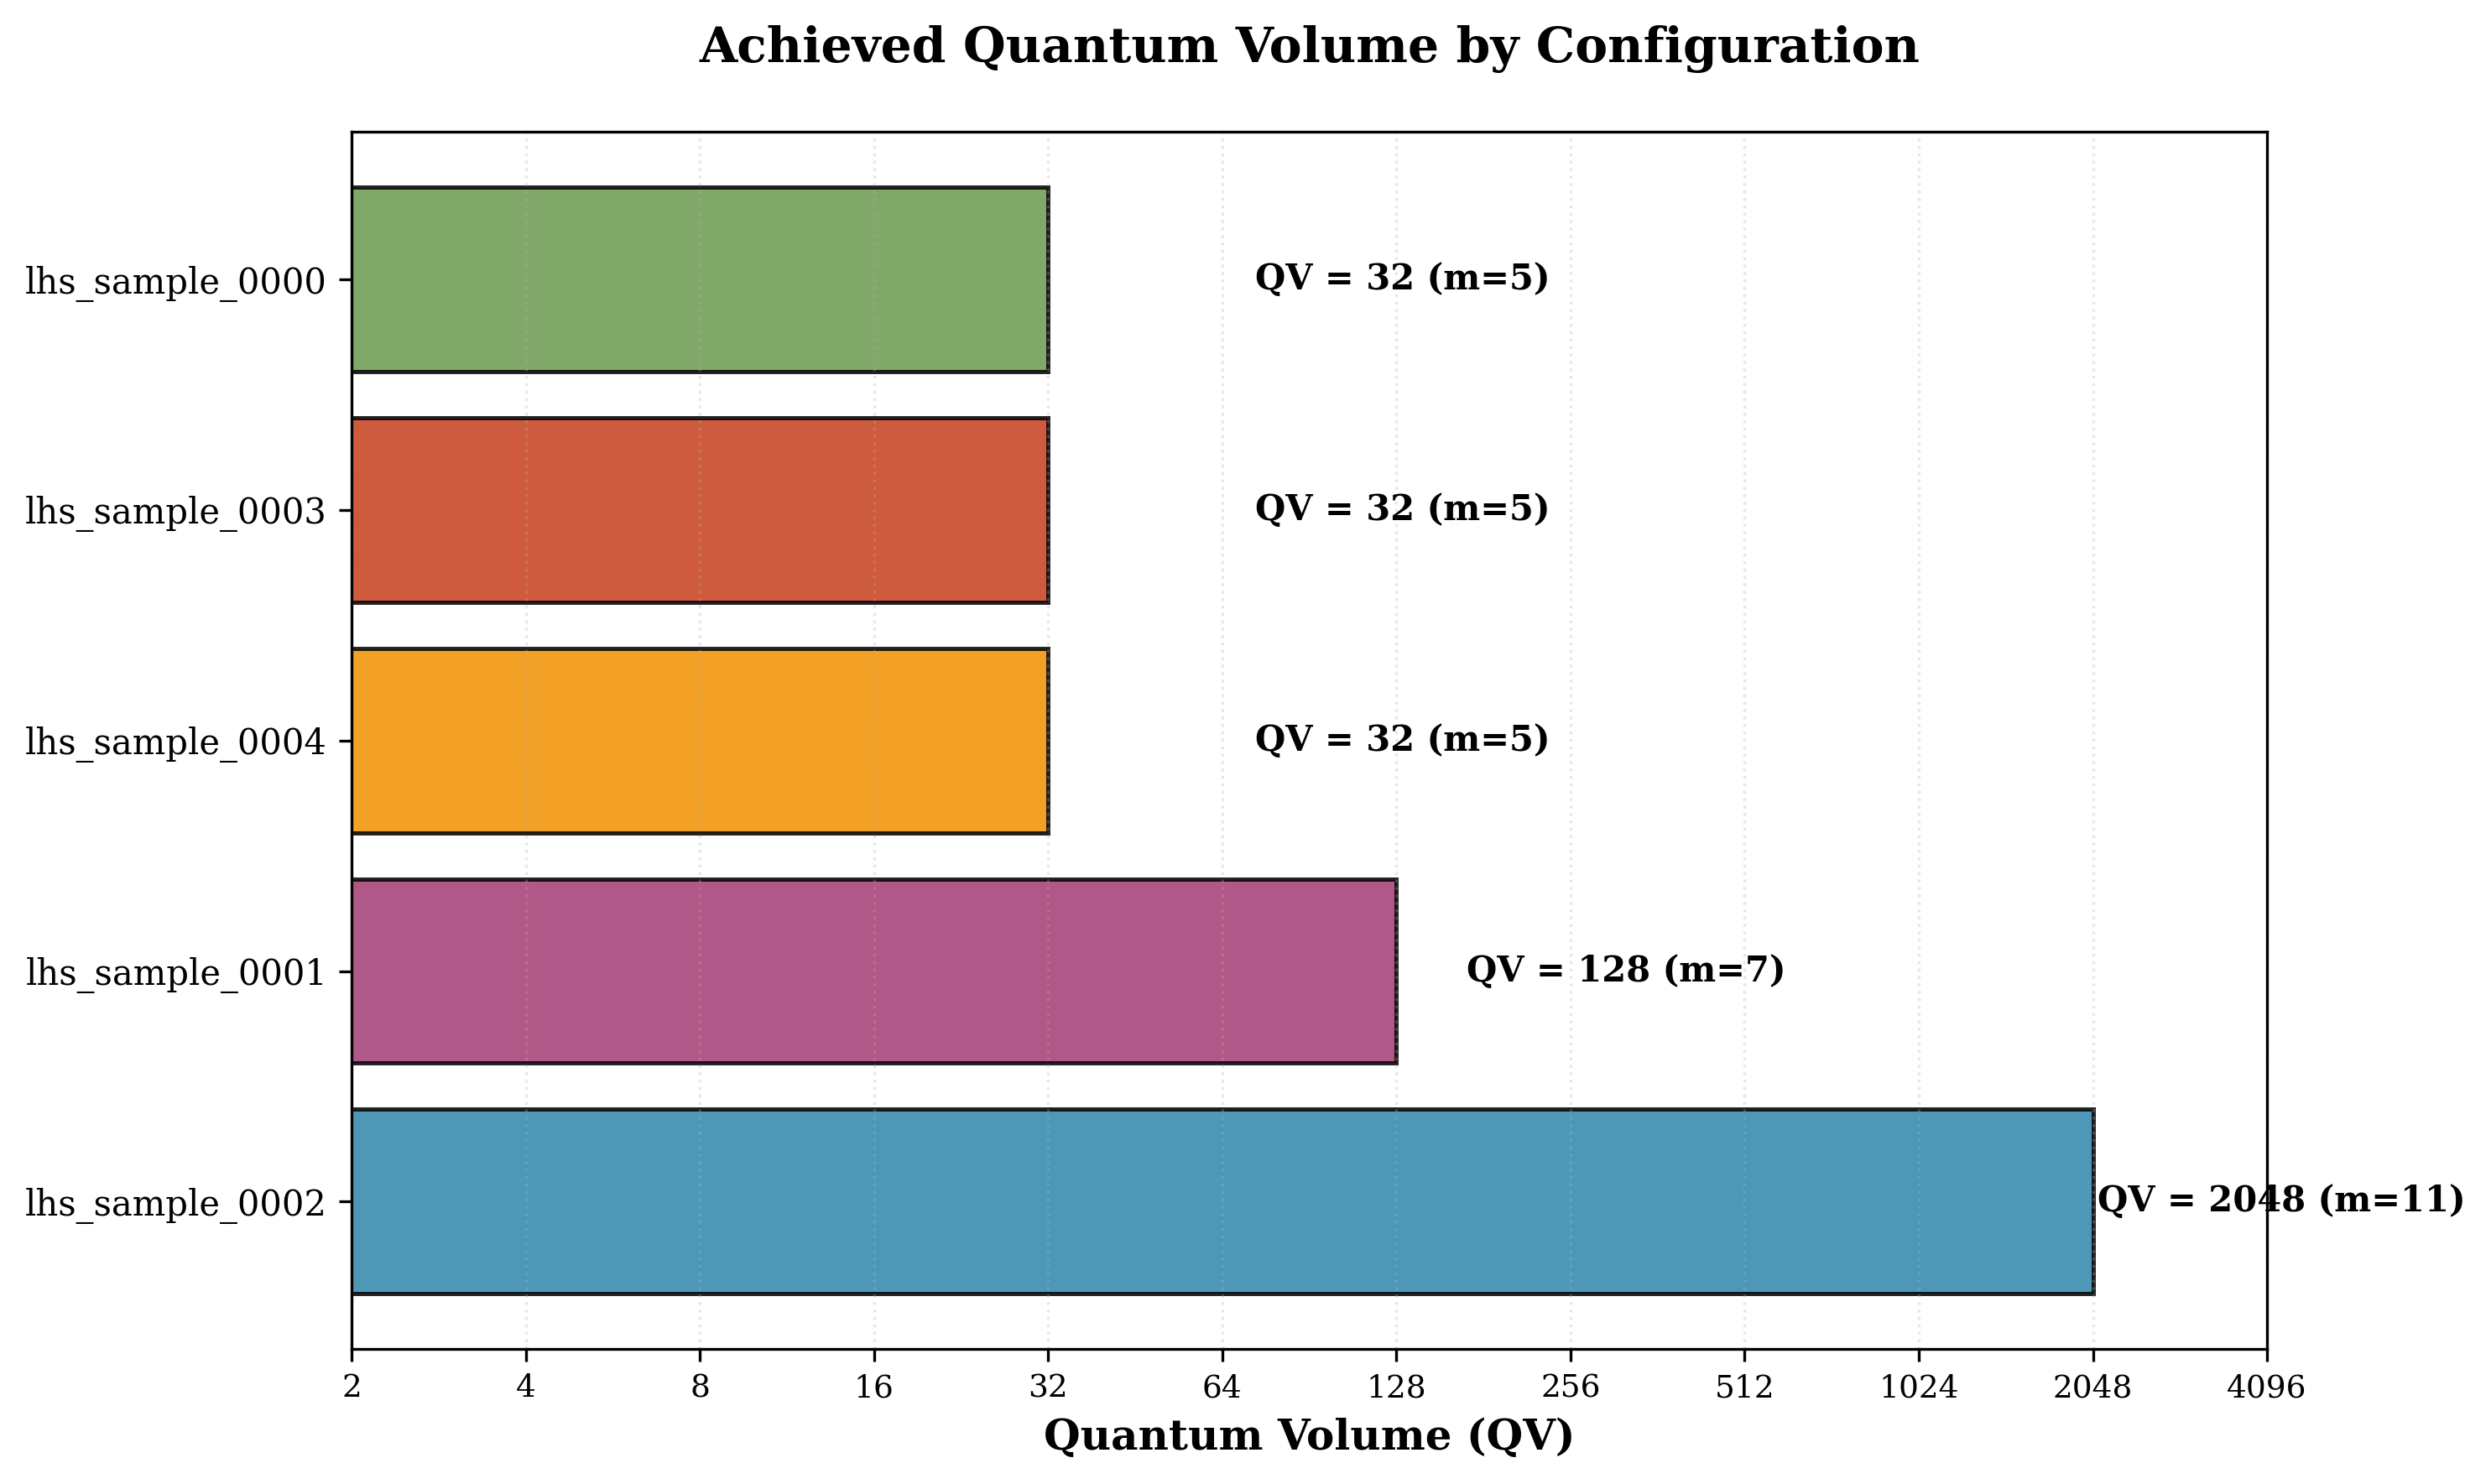
\includegraphics[width=0.85\linewidth]{plots/overview/achieved_qv_comparison.png}
  \caption{Achieved QV across LHS configurations (higher is better).}
  \label{fig:qv-overview}
\end{figure}

\begin{figure}[!htb]
  \centering
  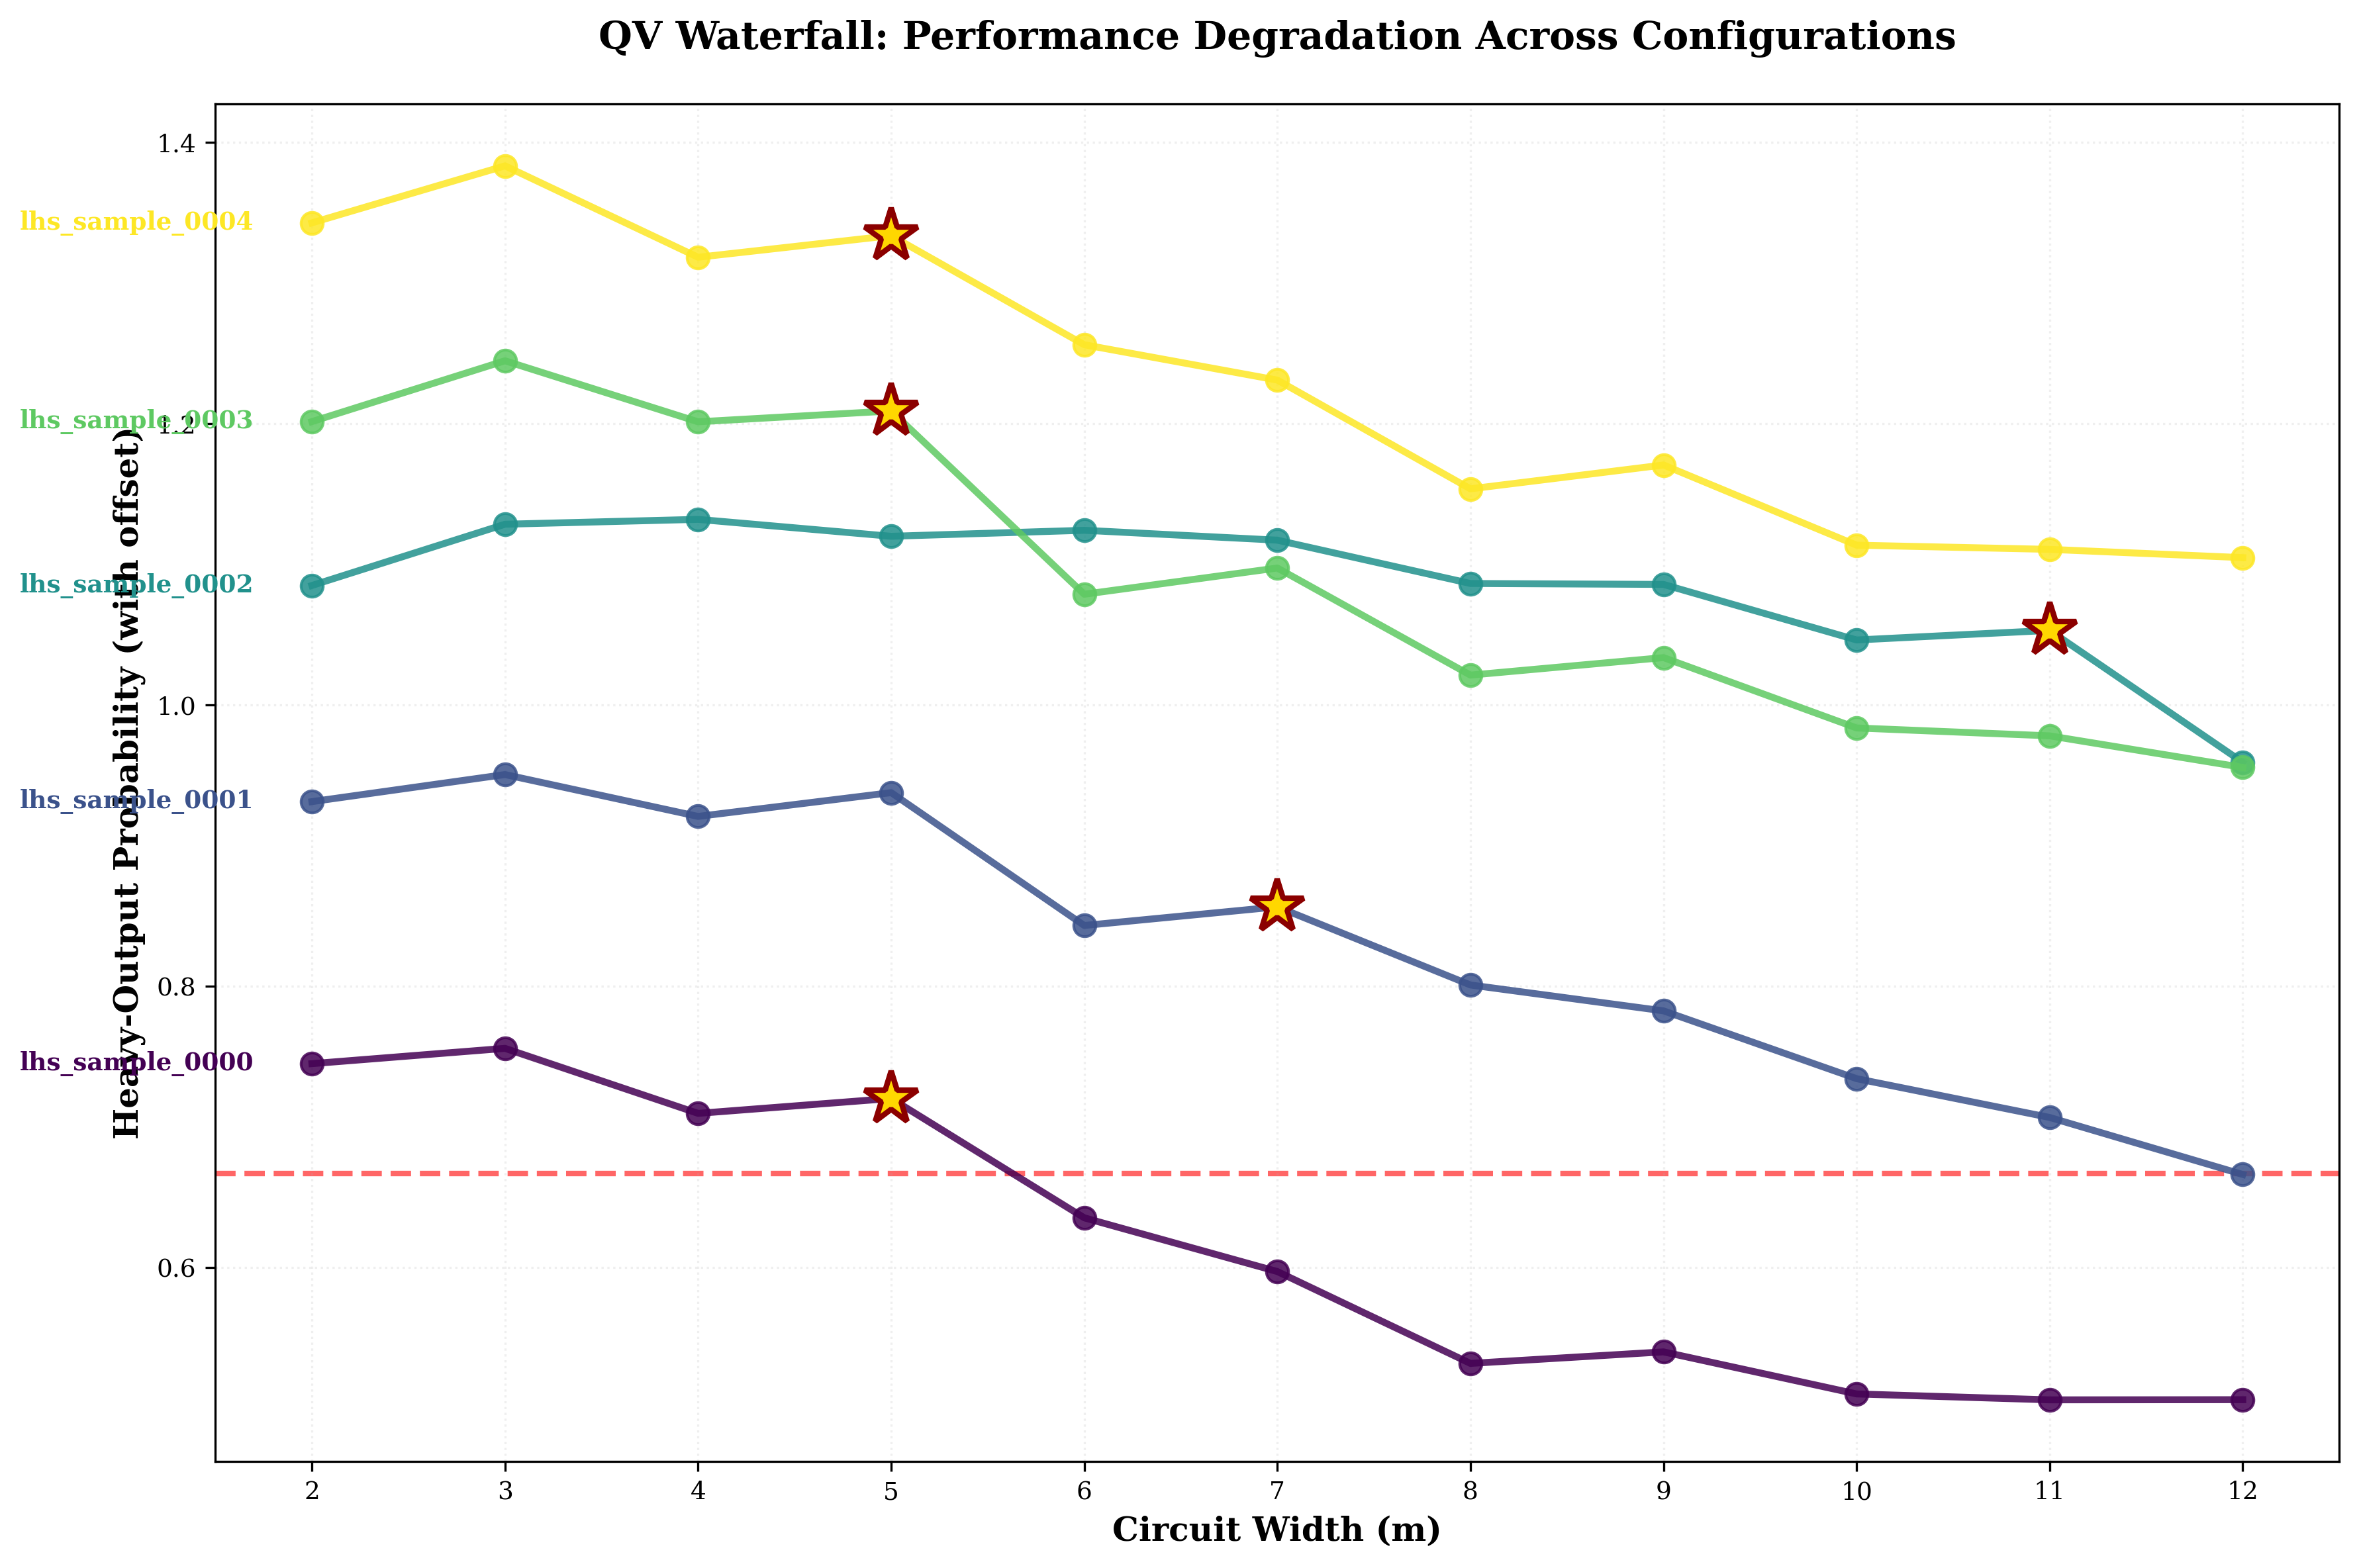
\includegraphics[width=0.85\linewidth]{plots/overview/qv_waterfall.png}
  \caption{QV waterfall by width $m$: heavy-output probability mean and 95\% CI vs threshold.}
  \label{fig:qv-waterfall}
\end{figure}

\subsection{Why lhs\_sample\_0002 achieved a higher QV}
Configuration \texttt{lhs\_sample\_0002} achieved $m^*=11$ ($\mathrm{QV}=2048$), substantially exceeding the other draws. The primary contributors are:
\begin{itemize}
  \item Two-qubit fidelity near the top of the sampled range: $F_2\approx0.99696$ gives $p_{2\mathrm{Q}}=\tfrac{4}{3}(1-F_2)\approx4.06\times10^{-3}$, an order of magnitude lower error than configurations with $F_2\approx0.93$--$0.96$.
  \item Long dephasing times: $T_2\approx2.5$\,ms and $T_2^*\approx16.8$\,$\mu$s reduce both Markovian phase damping during gates and quasi-static detuning per circuit; compare to $T_2^*\lesssim 6$\,$\mu$s in several other samples.
  \item Low measurement error: $P(0\mid1)\approx2.1\times10^{-3}$, which helps preserve HOP at larger widths where SPAM becomes increasingly consequential.
  \item Moderately low residual crosstalk: control crosstalk fraction $\approx1.22\%$ and ZZ-coupling $\sim10$\,kHz (lower than some samples with $\sim25$--$34$\,kHz), limiting coherent error accumulation through the deep, square QV circuits.
\end{itemize}
In combination, these factors keep the mean HOP and its lower 95\% CI above $2/3$ up to $m=11$. By contrast, configurations with lower $F_2$ (e.g., $F_2\approx0.93$) exhibit $p_{2\mathrm{Q}}\approx9.0\times10^{-2}$, leading to early failure at $m\approx5$ even when single-qubit fidelities are high.

\subsection{Connection to cited literature}
The sampled ranges for $F_1$, $F_2$, $T_1$, $T_2$, $T_2^*$, gate times, crosstalk, and SPAM are drawn from recent Si/SiGe spin-qubit reports (see main text references \cite{ref1,ref2,ref4,ref5,ref6,ref9,ref10,ref11}). The mapping from these physical metrics to quantum channels and coherent terms follows the conversion formulas listed above and is consistent with the simulator's unified, constrained error model.

\subsection{Reproducibility notes}
All widths used $N=100$ circuits and 5,000 shots per circuit with fixed RNG seeds per configuration. Backend was statevector with noisy channels applied as described. The JSON files \texttt{campaign\_manifest.json} and \texttt{campaign\_results.json}, together with the YAMLs in \texttt{latex/configs/}, capture the exact parameter draws and outcomes.




